\chapter{Modelo Proposto} \label{cpt:met_prop}
Este capítulo discorre sobre as etapas do desenvolvimento do LODUS-Health, uma ferramenta de simulação de fluxo de ocupação de leitos nos hospitais de Porto Alegre visando aprimorar a gestão hospitalar e urbana. A Figura~\ref{fig:metod} apresenta o fluxo de desenvolvimento da pesquisa, bem como o processo de execução do modelo final. Nas seções a seguir, são abordadas cada uma das etapas desse fluxo.

\begin{figure}
    \centering
    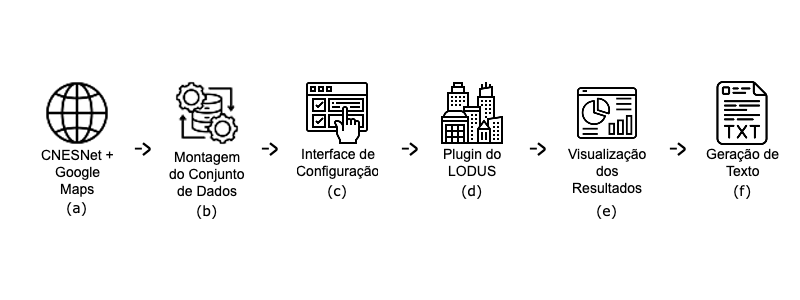
\includegraphics[width=\textwidth]{Capitulos/images/metodologia.png}
    \caption{Visão geral dos estágios de desenvolvimento do modelo.}
    \label{fig:metod}
\end{figure}

\section{CNESNet e Google Maps} \label{sec:sites}
A primeira etapa do fluxo de desenvolvimento representada pela Figura~\ref{fig:metod}(a) é a etapa de busca por dados de informações hospitalares em endereços eletrônicos para a montagem do conjunto de dados a ser utilizado na configuração do modelo de simulação. Foram utilizados os sites CNESNet\footnote{\url{https://cnes2.datasus.gov.br/}} e Google Maps\footnote{\url{https://www.google.com.br/maps/}} para essa busca. 
%SO: abaixo frase muito longa... revisar (GV: corrigido)

O CNESNet fornece acesso ao Cadastro Nacional de Estabelecimentos de Saúde (CNES), o sistema de informação oficial de cadastramento de informações de todos os estabelecimentos de saúde no país, sendo o cadastro oficial do Ministério da Saúde (MS), contendo informações relacionadas à capacidade instalada e mão de obra assistencial de saúde no Brasil em estabelecimentos de saúde públicos ou privados, com convênio SUS ou não, como forma de auxiliar no planejamento em saúde das três esferas de governo para uma gestão eficaz e eficiente~\cite{wikicnes}. 

O Google Maps oferece diversas funcionalidades relacionadas a mapas, incluindo visualização de mapas de ruas, rotas de navegação, informações de tráfego em tempo real, imagens de satélite, visualização em 360 graus de ruas (Street View) e informações sobre empresas locais, como restaurantes, lojas e serviços. Nesta pesquisa, utilizamos o CNESNet para obter informações relacionadas à quantidade de leitos por especialidade e tipo de leito nos hospitais de Porto Alegre e o Google Maps para recuperar informações geográficas de latitude e longitude dos hospitais.

Para a coleta dos dados, foi feita uma pesquisa no CNESNet em busca de informações sobre a quantidade de leitos disponíveis nos hospitais de Porto Alegre no mês de janeiro de 2024. Na página inicial dos resultados da pesquisa, está listada a relação da quantidade de leitos para cada especialidade, considerando o tipo de leito. A Figura~\ref{fig:cnesnet1} ilustra essas informações iniciais de leitos do tipo cirúrgico, onde a coluna ``Codigo'' refere-se a um identificador único da especialidade para o tipo de leito, ``Descrição'' descreve o nome da especialidade, ``Existente'' representa a quantidade total de leitos para a especialidade e, por fim, ``SUS'' se refere à quantidade de leitos SUS entre o número total de leitos.

\begin{figure}
    \centering
    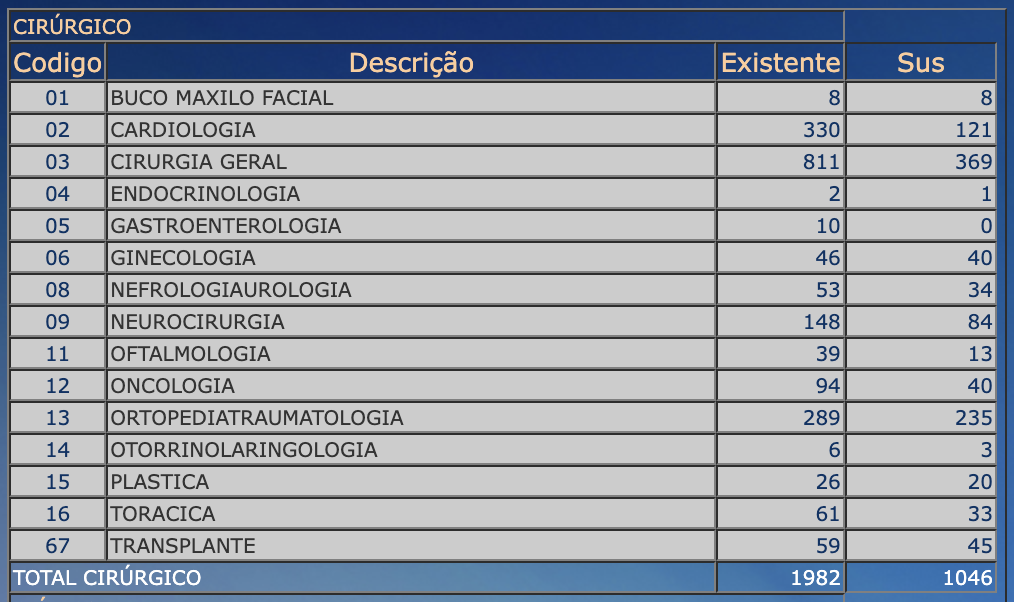
\includegraphics[width=\textwidth]{Capitulos/images/cnesnet1.png}
    \caption{Quantidade de leitos para especialidades do tipo ``cirúrgico'' nos hospitais de Porto Alegre/RS no mês de janeiro de 2024.}
    \label{fig:cnesnet1}
\end{figure}
%SO: sobre o caption da fig acima - colocar link dos dados. Fazer em todas as figs. (GV: revisar)

Para cada especialidade na lista, estão presentes informações sobre quais os hospitais que disponibilizam essa especialidade, a quantidade de leitos existentes e, dentre eles, quantos dos leitos são disponibilizados ao SUS, por fim, ao final da lista, apresenta-se o total de hospitais na cidade que disponibilizam essa especialidade de leito. A Figura~\ref{fig:cnesnet2} ilustra um exemplo dessas informações, onde a coluna ``CNES'' é o código identificador do cadastro do estabelecimento no sistema, ``Estabelecimento'' refere-se ao nome do hospital, ``Existente'' é a quantidade total de leitos para a especialidade e ``SUS'' é a quantidade de leitos SUS entre o número total de leitos.

\begin{figure}
    \centering
    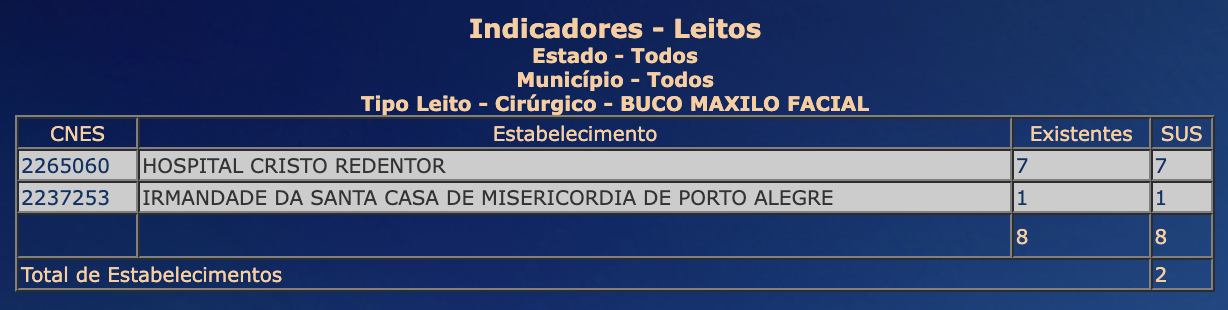
\includegraphics[width=\textwidth]{Capitulos/images/cnesnet2.png}
    \caption{Quantidade de leitos da especialidade ``Buco Maxilo Facial'' do tipo ``cirúrgico'' por hospital no mês de janeiro de 2024.}
    \label{fig:cnesnet2}
\end{figure}

Estes dados coletados serão utilizados como entradas em um conjunto de dados no qual cada hospital terá informações sobre suas especialidades por tipo de leito hospitalar. Após uma exploração nos dados disponíveis no CNESNet, foi decidido que, apesar de haver informações disponíveis sobre clínicas, nesta pesquisa consideraremos apenas os dados relacionados a hospitais, devido à baixa quantidade de leitos disponíveis e à complexidade de encontrar informações geográficas precisas sobre essas clínicas.

Por fim, a última etapa na coleta das informações para a criação do conjunto de dados ocorre na busca das coordenadas geográficas de cada hospital no Google Maps. É feita uma busca na ferramenta pelo nome do hospital (coluna ``Estabelecimento'' da Figura~\ref{fig:cnesnet2}) e recupera-se as informações de latitude e longitude de cada um deles. A Figura~\ref{fig:maps} mostra um exemplo da coleta desses dados utilizando o hospital São Lucas da PUCRS como referência, onde -30.05479 e -51.17142 são a latitude e longitude associadas, respectivamente.

\begin{figure}
    \centering
    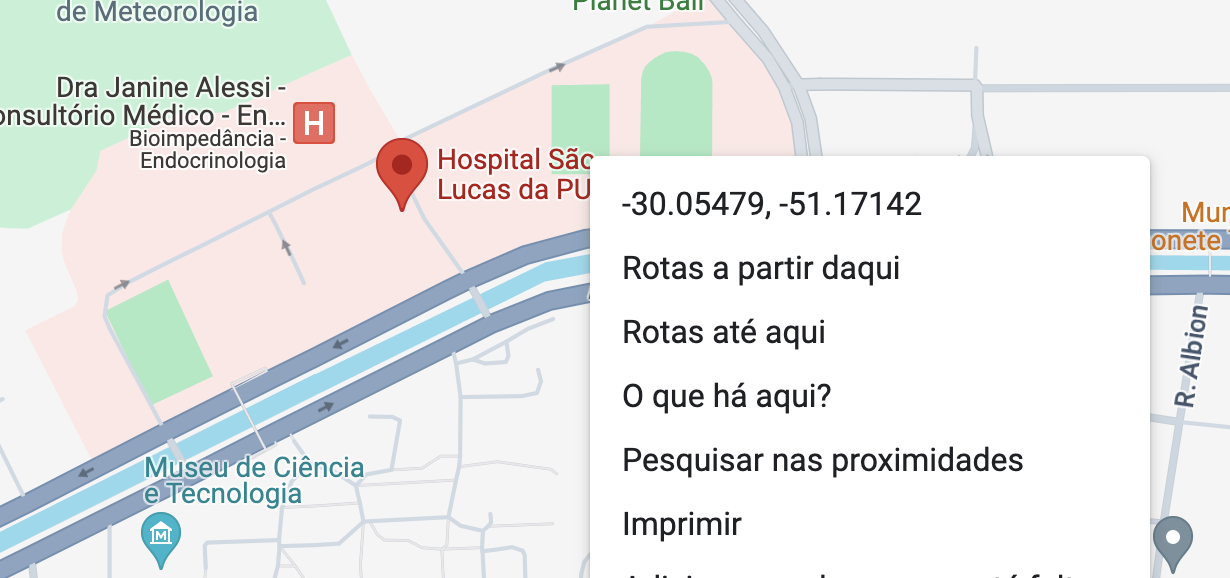
\includegraphics[width=0.97\textwidth]{Capitulos/images/maps.png}
    \caption{Busca pelas coordenadas geográficas de um hospital (latitude e longitude) no Google Maps.}
    \label{fig:maps}
\end{figure}

\section{Montagem do Conjunto de Dados}\label{sec:montagem_conjunto}
A montagem do conjunto de dados, representada na Figura~\ref{fig:metod}(b), é a etapa final na manipulação dos dados, etapa na qual ocorre a associação entre os dados recuperados nos endereços eletrônicos descritos na etapa anterior. O processo de montagem é realizado por meio da relação entre os dados dos hospitais e suas respectivas coordenadas. Para cada hospital recuperado no CNESNet, é associada uma coordenada no mapa (latitude e longitude), e as linhas do conjunto de dados são compostas pelas seguintes informações em um arquivo CSV:
%SO: coloquei em verbatim abaixo para ficar como dados de arquivo. coloca verbatim no parágrafo abauxo do item itemze em cada palavra
\begin{itemize}
    \item \begin{verbatim}LAT\end{verbatim}
    \item \begin{verbatim}LONG\end{verbatim}
    \item \begin{verbatim}HOSPITAL\end{verbatim}
    \item \begin{verbatim}REGIAO\end{verbatim}
    \item \begin{verbatim}DESCRICAO\end{verbatim}
    \item \begin{verbatim}TIPO\end{verbatim}
    \item \begin{verbatim}TOTAL\end{verbatim}
    \item \begin{verbatim}SUS\end{verbatim}
\end{itemize}
    
As colunas ``LAT'' e ``LONG'' referem-se às coordenadas geográficas de onde o hospital está localizado no mapa, ``HOSPITAL'' é o nome do hospital, ``REGIAO'' é o bairro onde o hospital está situado, ``DESCRICAO'' é a especialidade do leito do hospital, ``TIPO'' é o tipo de leito hospitalar, ``TOTAL'' é a quantidade total de leitos para a especialidade e ``SUS'' é a quantidade de leitos disponíveis para SUS entre o total de leitos. A Tabela~\ref{table:3} ilustra um exemplo dessa estrutura de entradas do conjunto de dados apresentando informações do hospital HPS. 
%SO: verbatim abaixo tb
\begin{table}[h!]
\centering
\begin{tabular}{ |c|c|c|c|c|c|c|c| } 
 \hline
 \verb|LAT| & \verb|LONG| & \verb|HOSPITAL| & \verb|REGIAO| & \verb|DESCRICAO| & \verb|TIPO| & \verb|TOTAL| & \verb|SUS|\\ 
 \hline
 \verb|-30.036...| & \verb|-51.211...| & \verb|HPS| & \verb|Bom Fim| & \verb|Cirurgia Geral| & \verb|Cirúrgico| & \verb|21| & \verb|21|\\  \hline
 \verb|-30.036...| & \verb|-51.211...| & \verb|HPS| & \verb|Bom Fim| & \verb|Neurocirurgia| & \verb|Cirúrgico| & \verb|15| & \verb|15|\\
 \hline
\end{tabular}
\caption{Exemplo de entradas do conjunto de dados criado.}
\label{table:3}
\end{table}

\subsection{Análise do Conjunto de Dados}
Concluída a etapa de montagem do conjunto de dados, os dados estão prontos para serem utilizados na pesquisa. Para isso, inicialmente utilizamos a aplicação web Jupyter Notebook\footnote{\url{https://docs.jupyter.org/en/latest/}} disponível através do Google Colab\footnote{\url{https://colab.research.google.com/}} %SO: link (FEITO)
para a realização de uma análise sobre os dados e entender a distribuição das informações dos hospitais no conjunto de dados. O desenvolvimento da exploração e análise dos dados foi realizado utilizando a linguagem Python\footnote{\url{https://docs.python.org/3/}}, juntamente com a biblioteca de manipulação e análise de dados Pandas\footnote{\url{https://pandas.pydata.org/docs/}}, dentro da aplicação web Jupyter Notebook, uma aplicação web utilizada para criar e compartilhar documentos computacionais~\cite{JUPYTER}. 

O conjunto de dados final resultou em um arquivo contendo 254 entradas, cada uma representando informações de leitos hospitalares para uma determinada especialidade, conforme apresentado anteriormente. Foram recuperadas ao todo informações de 28 hospitais no CNESNet, distribuídos em 22 bairros de Porto Alegre, abrangendo um total de 48 especialidades de leitos distintos. Além disso, foram identificados 7 tipos de leitos distintos (``cirúrgico'', ``clínico'', ``obstétrico'', etc.). Ao total, estão disponíveis informações de 7.529 leitos hospitalares, dos quais 4.689 leitos estão disponíveis para o SUS, representando aproximadamente 62,27\% dos leitos dos hospitais selecionados.

No gráfico da Figura~\ref{fig:graph1}, destacam-se os 10 hospitais com as maiores diversidades de especialidades de leitos. Entre eles, os hospitais com o maior número de especialidades distintas são o Hospital Nossa Senhora da Conceição, a Irmandade da Santa Casa de Misericórdia de Porto Alegre e o Hospital Divina Providência, contendo 31, 30 e 24 especialidades de leitos, respectivamente.

\begin{figure}
    \centering
    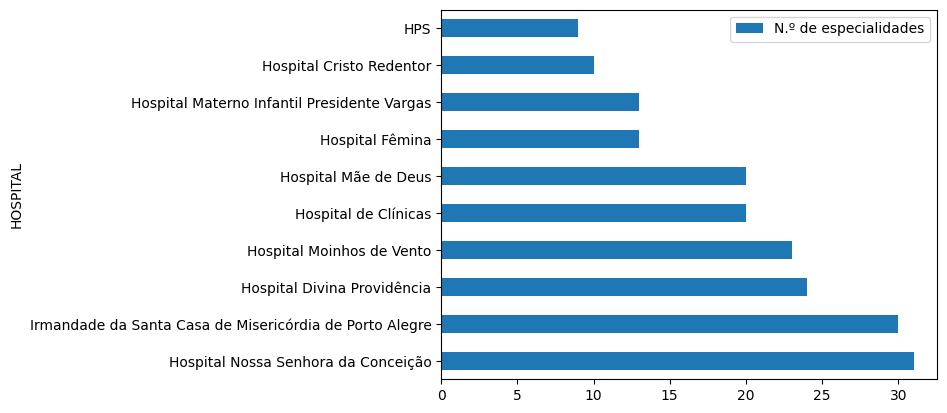
\includegraphics[width=\textwidth]{Capitulos/images/graph1.png}
    \caption{Os 10 hospitais selecionados com o maior número de especialidades distintas.}
    \label{fig:graph1}
\end{figure}

Já os 10 hospitais com os maiores números de leitos disponíveis (Figura~\ref{fig:graph2}) são a Irmandade da Santa Casa de Misericórdia de Porto Alegre, com 1.066 leitos, o Hospital Nossa Senhora da Conceição, com 912, e o Hospital de Clínicas, com 885 leitos disponíveis. Observando a Figura~\ref{fig:graph2}, em termos de quantidade de leitos SUS, os hospitais Nossa Senhora da Conceição, com 912 leitos, Hospital de Clínicas, com 747, e Associação Hospitalar Vila Nova, com 637, são os que possuem maior disponibilidade para leitos públicos. De maneira geral, os leitos hospitalares tem uma disponibilidade equilibrada entre privados e SUS. No entanto, observa-se a presença de hospitais que não oferecem atendimento SUS, como os hospitais Mãe de Deus, Ernesto Dornelles e Moinhos de Vento. Além disso, há hospitais que têm toda ou a maior parte de sua capacidade dedicada ao SUS, como o Hospital de Clínicas, com cerca de 84\%, a Associação Hospitalar Vila Nova, com cerca de 99\% de sua capacidade, e o hospital Nossa Senhora da Conceição, com 100\% da capacidade dedicada.

\begin{figure}
    \centering
    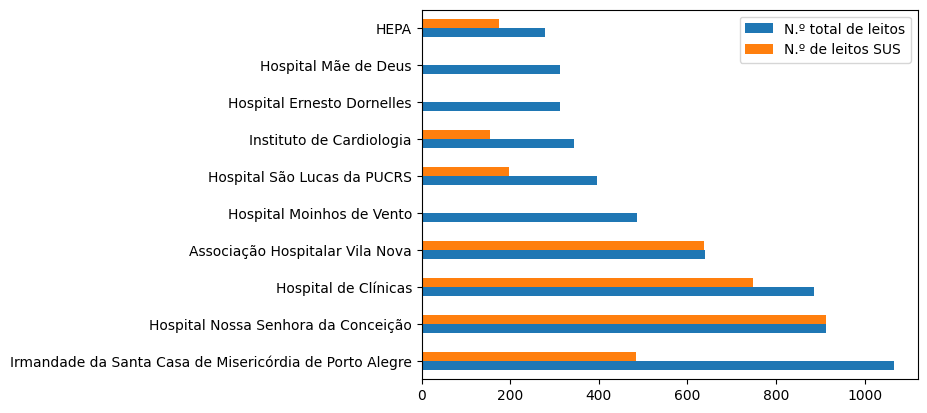
\includegraphics[width=\textwidth]{Capitulos/images/graph2.png}
    \caption{Os 10 hospitais selecionados com o maior número de leitos, separados entre total e SUS.}
    \label{fig:graph2}
\end{figure}

Seguindo a análise do conjunto de dados, a Figura~\ref{fig:graph3} apresenta as 10 especialidades mais frequentes nos leitos dos hospitais de Porto Alegre. As especialidades de ``Cirurgia Geral'', do tipo ``Cirúrgico'', e ``Clínica Geral'', do tipo ``Clínico'', são as mais comuns nos hospitais da cidade, presentes em 18 hospitais cada. Em seguida, a especialidade ``UTI Adulto - Tipo III'', do tipo de leito ``Complementar'', está presente em 12 hospitais dos 28 hospitais selecionados.

\begin{figure}
    \centering
    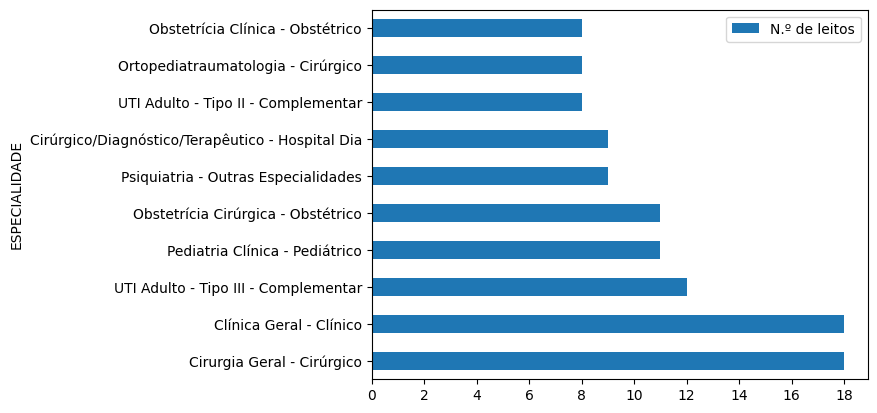
\includegraphics[width=\textwidth]{Capitulos/images/graph3.png}
    \caption{As 10 especialidades mais frequentes nos leitos dos hospitais selecionados.
    %GA: Os dados não tem falores float, certo? caso não, ajustar o exito X para ser valores inteiros (GV: corrigido)
    }
    \label{fig:graph3}
\end{figure}

Feitas as análises que complementam a busca e o armazenamento estruturado dos dados, parte-se para a apresentação dos processo de interação e simulação.

\section{Interface de Configuração}\label{sec:interface_config}
A interface gráfica de configuração (representada na Figura~\ref{fig:metod}(c))
%SO: conferir se é mesmo (c). quando falar das partes da fig1, mencionar a letrinha (GV: revisar)
neste estudo foi desenvolvida com o objetivo de facilitar a parametrização dos dados de entrada do modelo de simulação. Além disso, espera-se tornar o uso do simulador mais acessível para pessoas de fora da área da tecnologia, eliminando a necessidade do usuário de criar arquivos em formatos comuns para profissionais de computação, como por exemplo JSON e CSV.

A tecnologia central empregada no desenvolvimento da interface foi o Flask\footnote{\url{https://flask.palletsprojects.com/en/3.0.x/}}, um \textit{framework} escrito em Python voltado para o desenvolvimento web. Essa tecnologia é crucial para estabelecer a conexão entre os parâmetros do usuário e a execução do LODUS a partir deles. Além disso, outras tecnologias foram utilizadas no desenvolvimento da interface. Utilizamos HTML, CSS e Bootstrap\footnote{\url{https://getbootstrap.com/docs/4.6/getting-started/introduction/}} para estilizar a interface e tornar sua utilização amigável, JavaScript para auxiliar na lógica de programação e também na conexão com o código do LODUS, e o Plotly\footnote{\url{https://plotly.com/}
} na apresentação dos resultados da simulação utilizando um mapa \textit{choropleth}. As tecnologias utilizadas no estudo foram selecionadas devido à familiaridade dos pesquisadores.

A interface foi desenvolvida para abranger três funcionalidades principais: permitir a configuração dos parâmetros do modelo de simulação, possibilitando o uso de dados reais de hospitais provenientes do DATASUS\footnote{\url{https://datasus.saude.gov.br/}}, disponíveis no CNESNet ou que o usuário crie dados fictícios, facilitando a execução do simulador para diversos tipos de usuários; apresentar os resultados obtidos na simulação de forma clara e objetiva; e permitir que o usuário escolha especialidades de leitos para a geração de textos no contexto desejado. Nesta seção, será abordada a etapa de configuração dos parâmetros do modelo de simulação.

Para que o usuário fosse capaz de configurar a parametrização do modelo de simulação, foi criada uma interface (Figura~\ref{fig:simul1}) que permite a entrada de parâmetros como o título da simulação (Figura~\ref{fig:simul1}(a)), período de simulação em dias e horas (Figura~\ref{fig:simul1}(b)), os quais serão contabilizados como passos de simulação, 
%SO: ficou essa troca? (GV: corrigido)
escolha ou criação de hospitais a serem simulados (Figura~\ref{fig:simul1}(c)), e a listagem dos hospitais selecionados (Figura~\ref{fig:simul1}(d)), possibilitando a configuração e remoção de cada um deles.

\begin{figure}
    \centering
    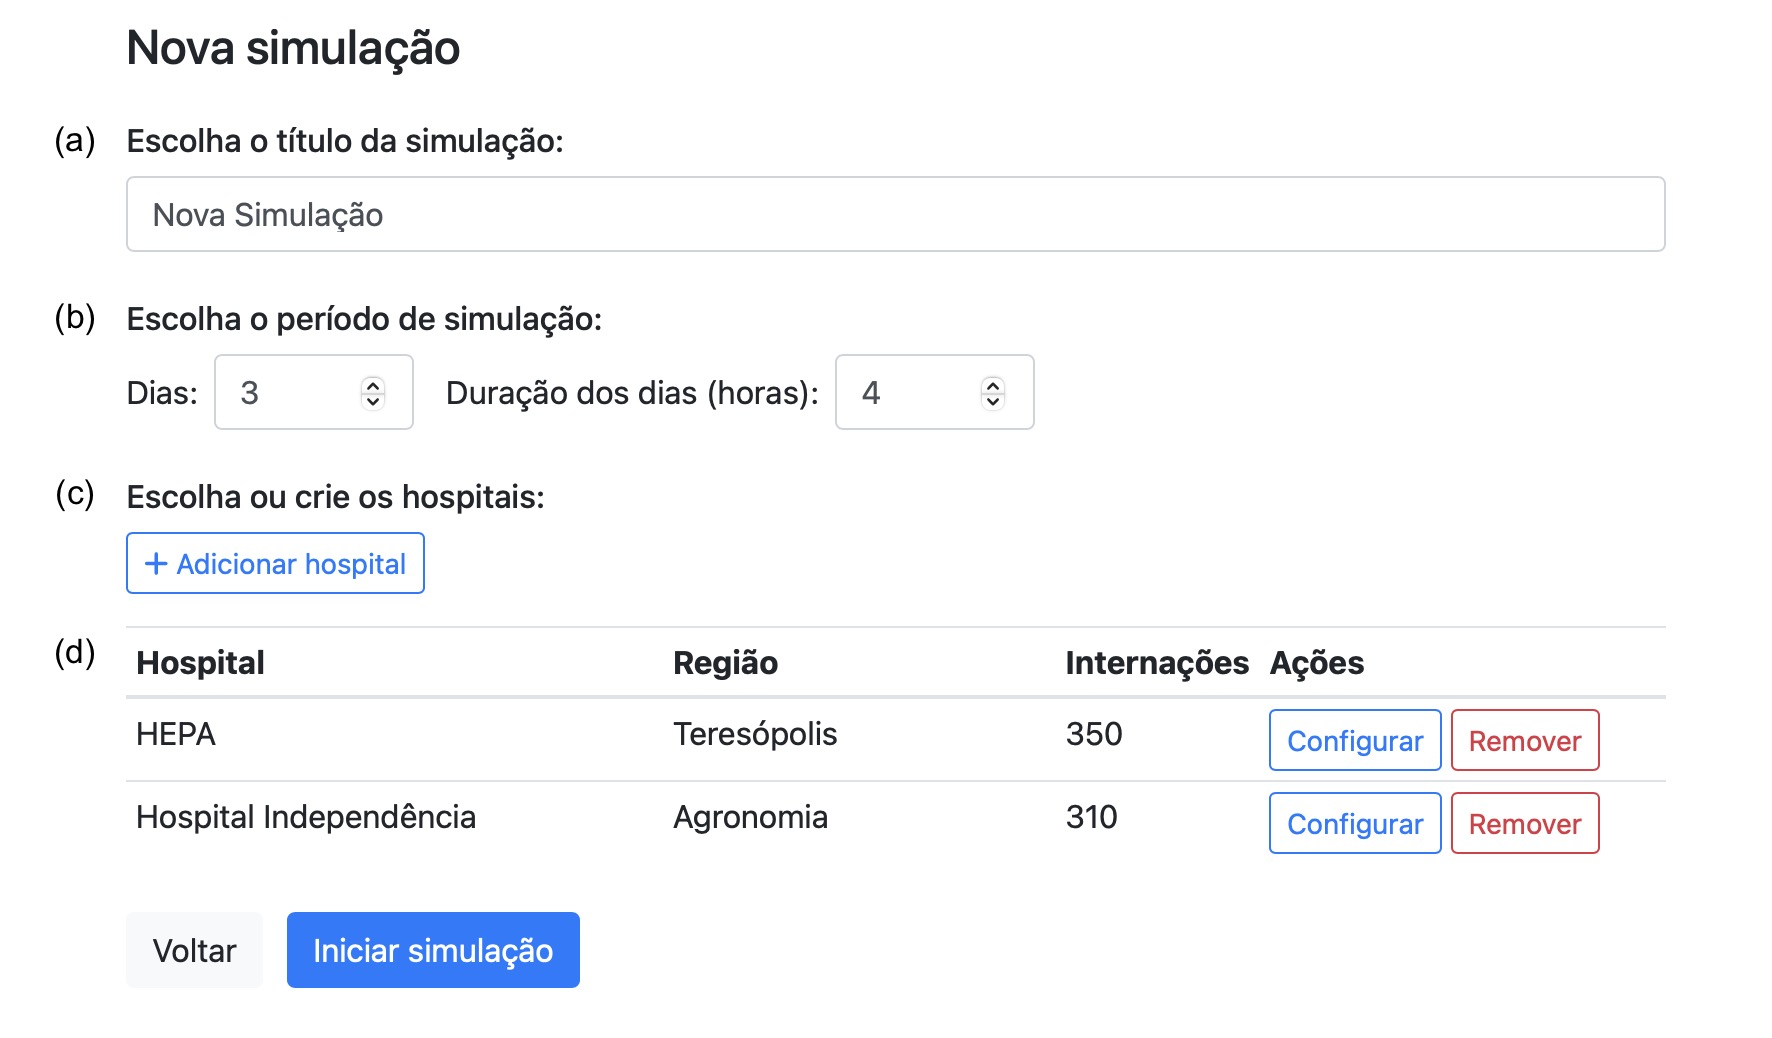
\includegraphics[width=\textwidth]{Capitulos/images/simul1.jpeg}
    \caption{Tela de configuração dos parâmetros de simulação.}
    \label{fig:simul1}
\end{figure}

Ao usuário selecionar a opção ``Adicionar hospital'' (Figura~\ref{fig:simul1}(c)), aparecem opções de parametrização relacionadas à criação ou seleção de um hospital a ser utilizado na simulação. Nessa tela (Figura~\ref{fig:simul2}), o usuário pode escolher um hospital a partir de dados provenientes do conjunto de dados apresentado na seção anterior (Figura~\ref{fig:simul2}(a)), ou criar um novo hospital (Figura~\ref{fig:simul2}(b)), adicionar especialidades de leitos a partir dos dados do CNESNet (Figura~\ref{fig:simul2}(c)), criar uma nova especialidade (Figura~\ref{fig:simul2}(d)), ou listar as especialidades selecionadas com a possibilidade de remover as indesejadas (Figura~\ref{fig:simul2}(e)).

\begin{figure}
    \centering
    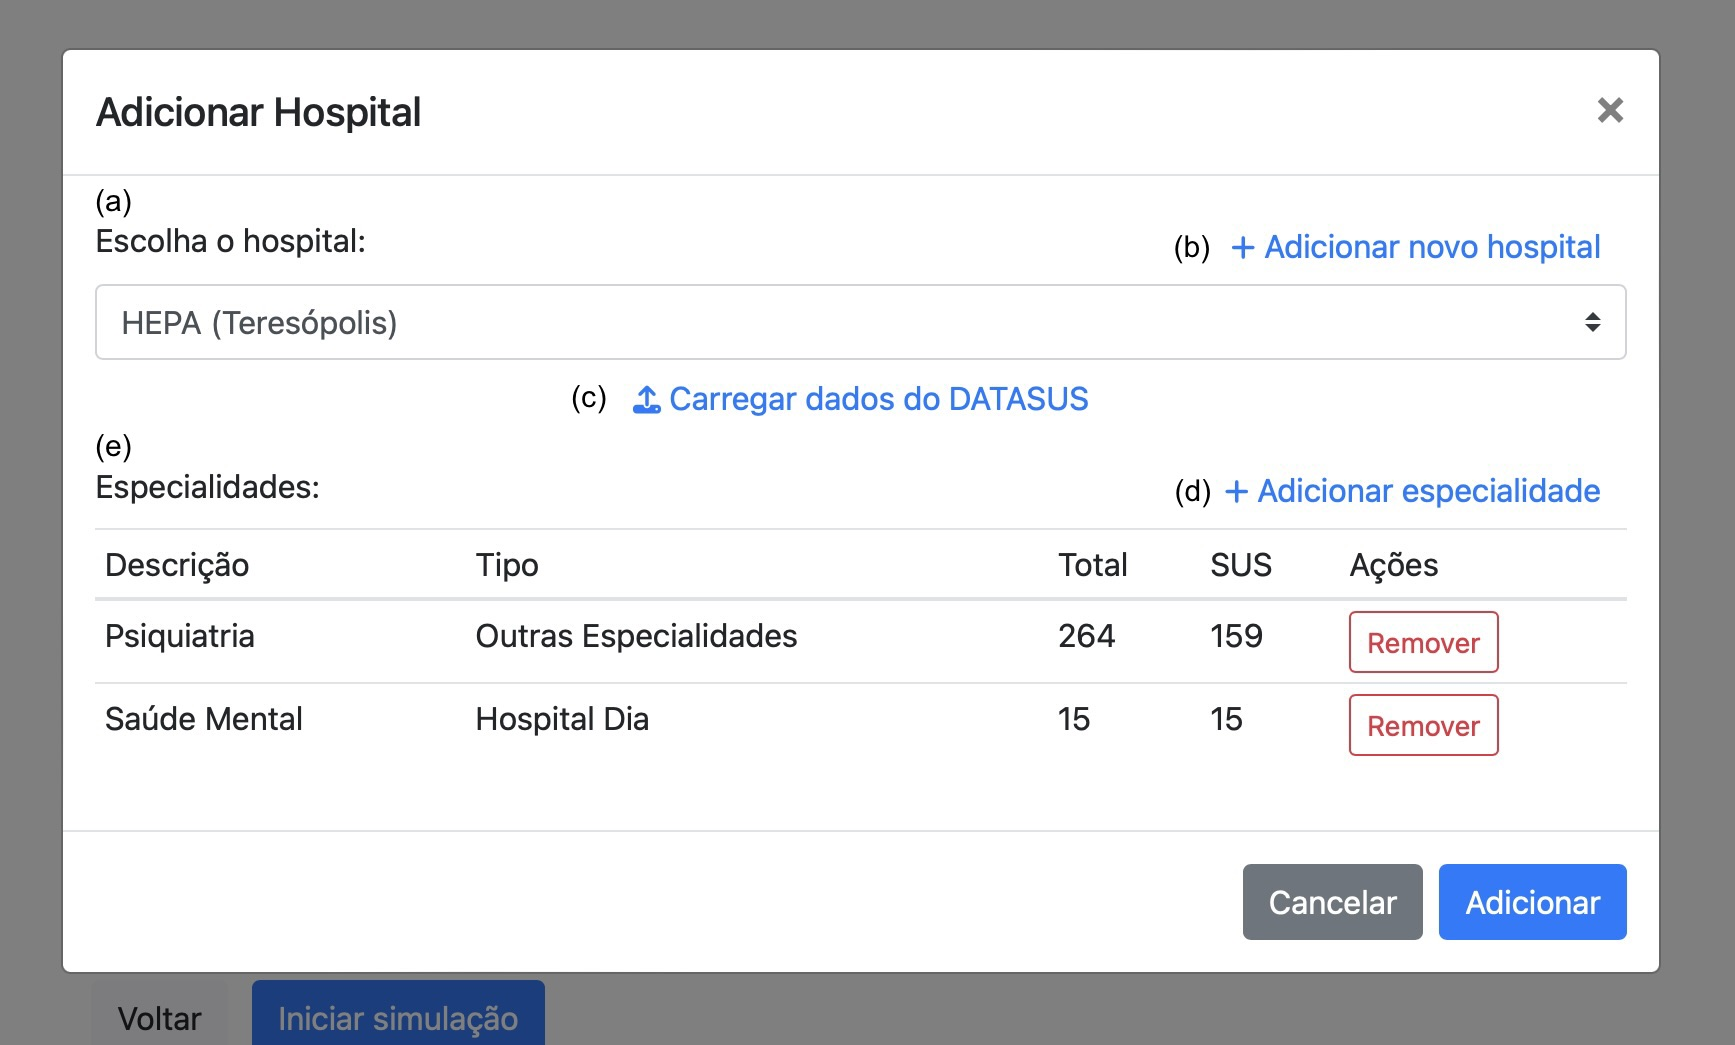
\includegraphics[width=\textwidth]{Capitulos/images/simul2.jpeg}
    \caption{Tela de seleção de hospital um hospital para a simulação.}
    \label{fig:simul2}
\end{figure}

Ao selecionar ``Adicionar novo hospital'' (Figura~\ref{fig:simul2}(b)), o usuário tem a opção de inserir um novo hospital para escolha na configuração da simulação (Figura~\ref{fig:simul3}), para isso, o usuário deve informar o nome do hospital (Figura~\ref{fig:simul3}(a)), selecionar a região (bairro) à qual ele pertence (Figura~\ref{fig:simul3}(b)) e definir as coordenadas geográficas (latitude e longitude) do mesmo (Figura~\ref{fig:simul3}(c)).

\begin{figure}
    \centering
    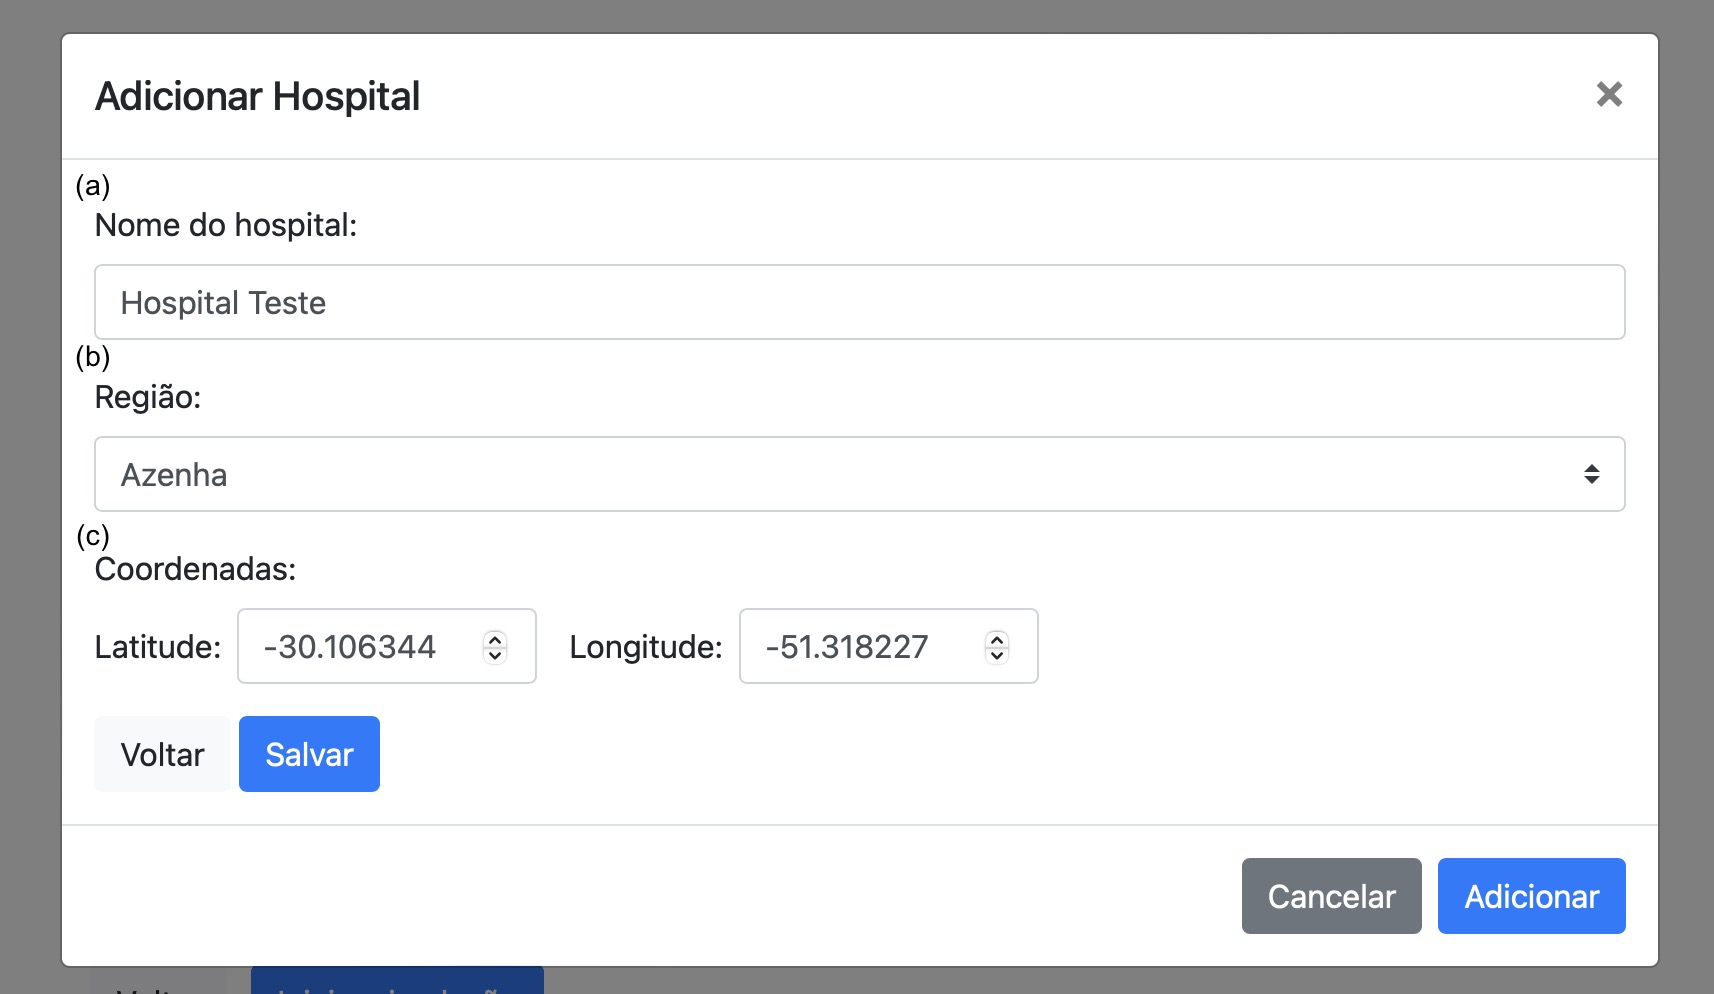
\includegraphics[width=\textwidth]{Capitulos/images/simul3.jpeg}
    \caption{Tela de criação de uma opção de hospital para a simulação.}
    \label{fig:simul3}
\end{figure}

Após a seleção ou criação de um hospital, o usuário pode personalizar suas características, podendo selecionar diversas especialidades dentre as já existentes ou criar uma nova especialidade de leito customizada (Figura~\ref{fig:simul4}). Para isso, deve-se informar o nome da especialidade (Figura~\ref{fig:simul4}(a)). Se ela já existir, o usuário seleciona na lista; caso contrário, deve-se informar o nome, o tipo de leito (Figura~\ref{fig:simul4}(b)), e a quantidade total de leitos disponíveis e dentre os leitos disponíveis, a quantidade dedicada para o SUS (Figura~\ref{fig:simul4}(c)).

\begin{figure}
    \centering
    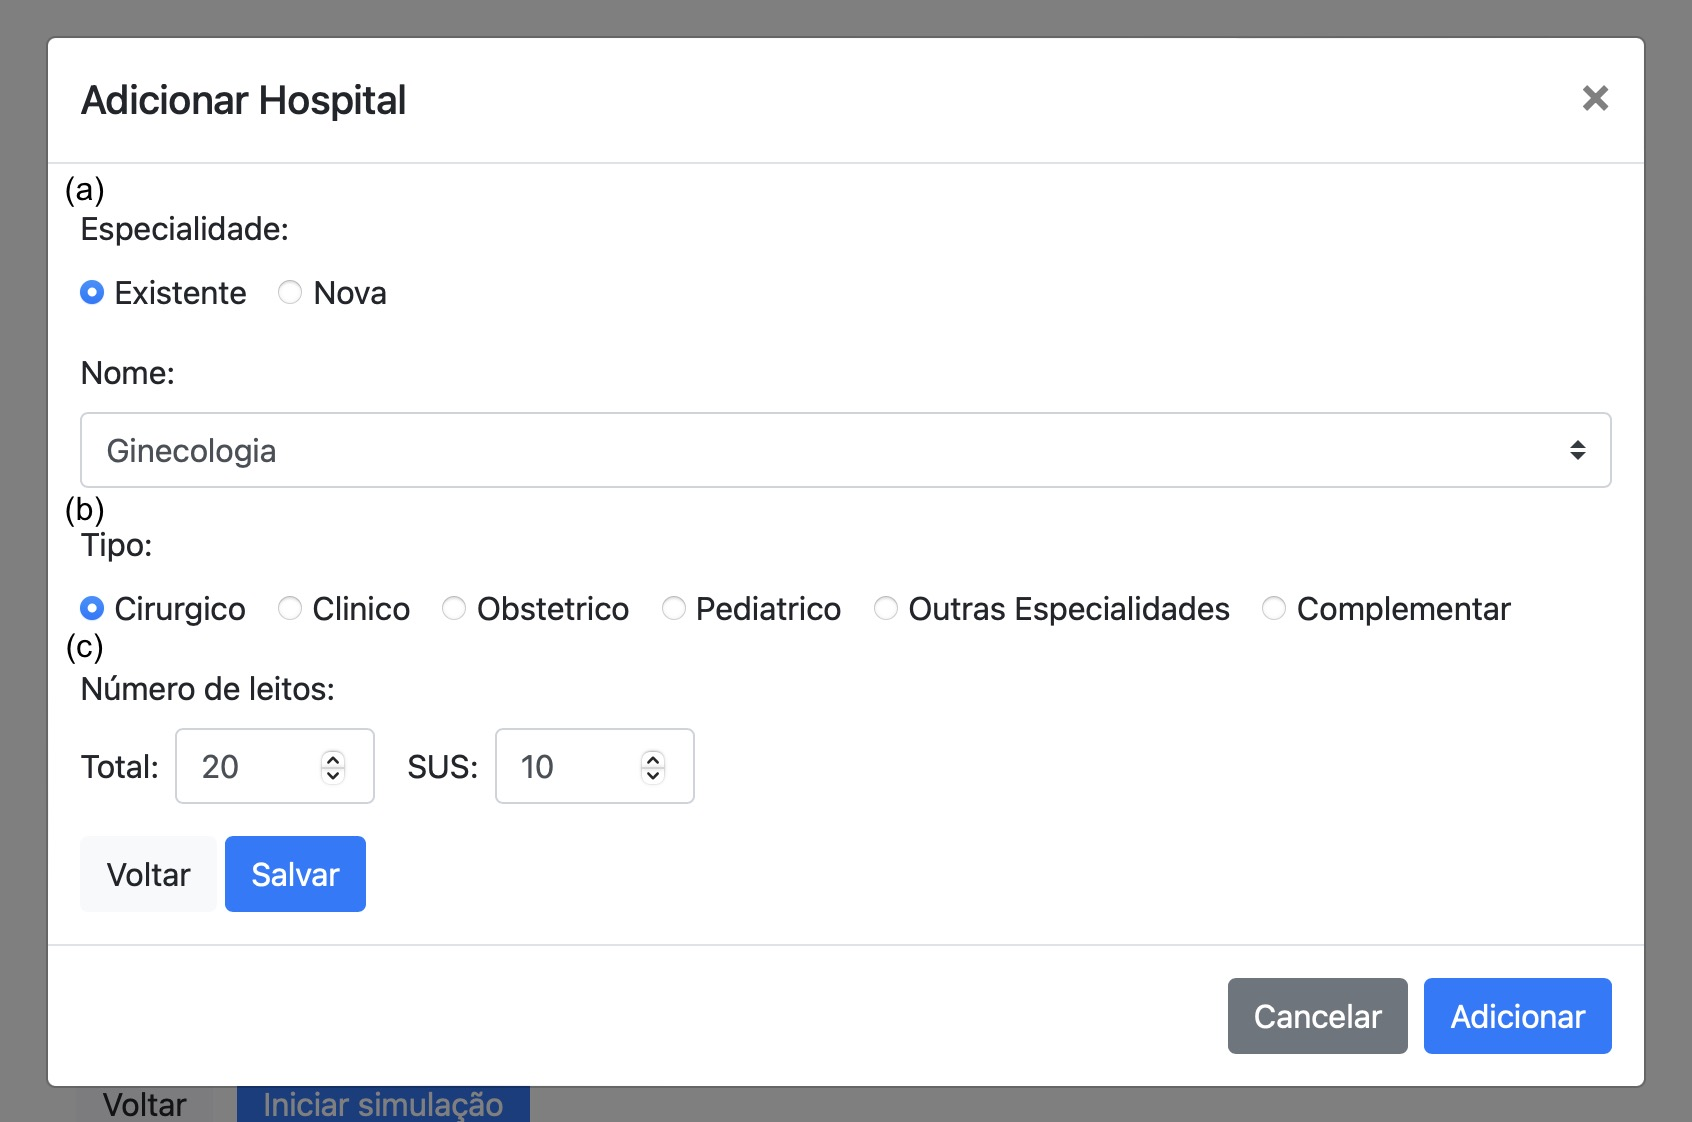
\includegraphics[width=\textwidth]{Capitulos/images/simul4.jpeg}
    \caption{Tela de criação de uma especialidade.}
    \label{fig:simul4}
\end{figure}

Por fim, a última ação do usuário na criação dos parâmetros de simulação é a definição das chamadas de pacientes para hospitais na simulação (Figura~\ref{fig:simul5}). Informa-se quantos pacientes serão internados para uma especialidade específica no período de simulação definido na tela inicial (Figura~\ref{fig:simul5}(a)), quantas internações serão destinadas ao SUS (Figura~\ref{fig:simul5}(b)) e por quantos passos de simulação, em média, os internados naquela especialidade permanecem no leito hospitalar na simulação, definindo o número mínimo e máximo de passos (Figura~\ref{fig:simul5}(c)). Por exemplo, na Figura~\ref{fig:simul5}, o hospital HEPA possui 264 leitos da especialidade ``Psiquiatria'' do tipo ``Outras Especialidades'', sendo 159 deles disponíveis para o SUS. Foi informado que durante o período de simulação serão utilizados 500 leitos para pacientes, sendo 300 em leitos do SUS. Também foi parametrizado que um paciente pode permanecer em média de 1 a 4 passos de simulação ocupando o leito.

\begin{figure}
    \centering
    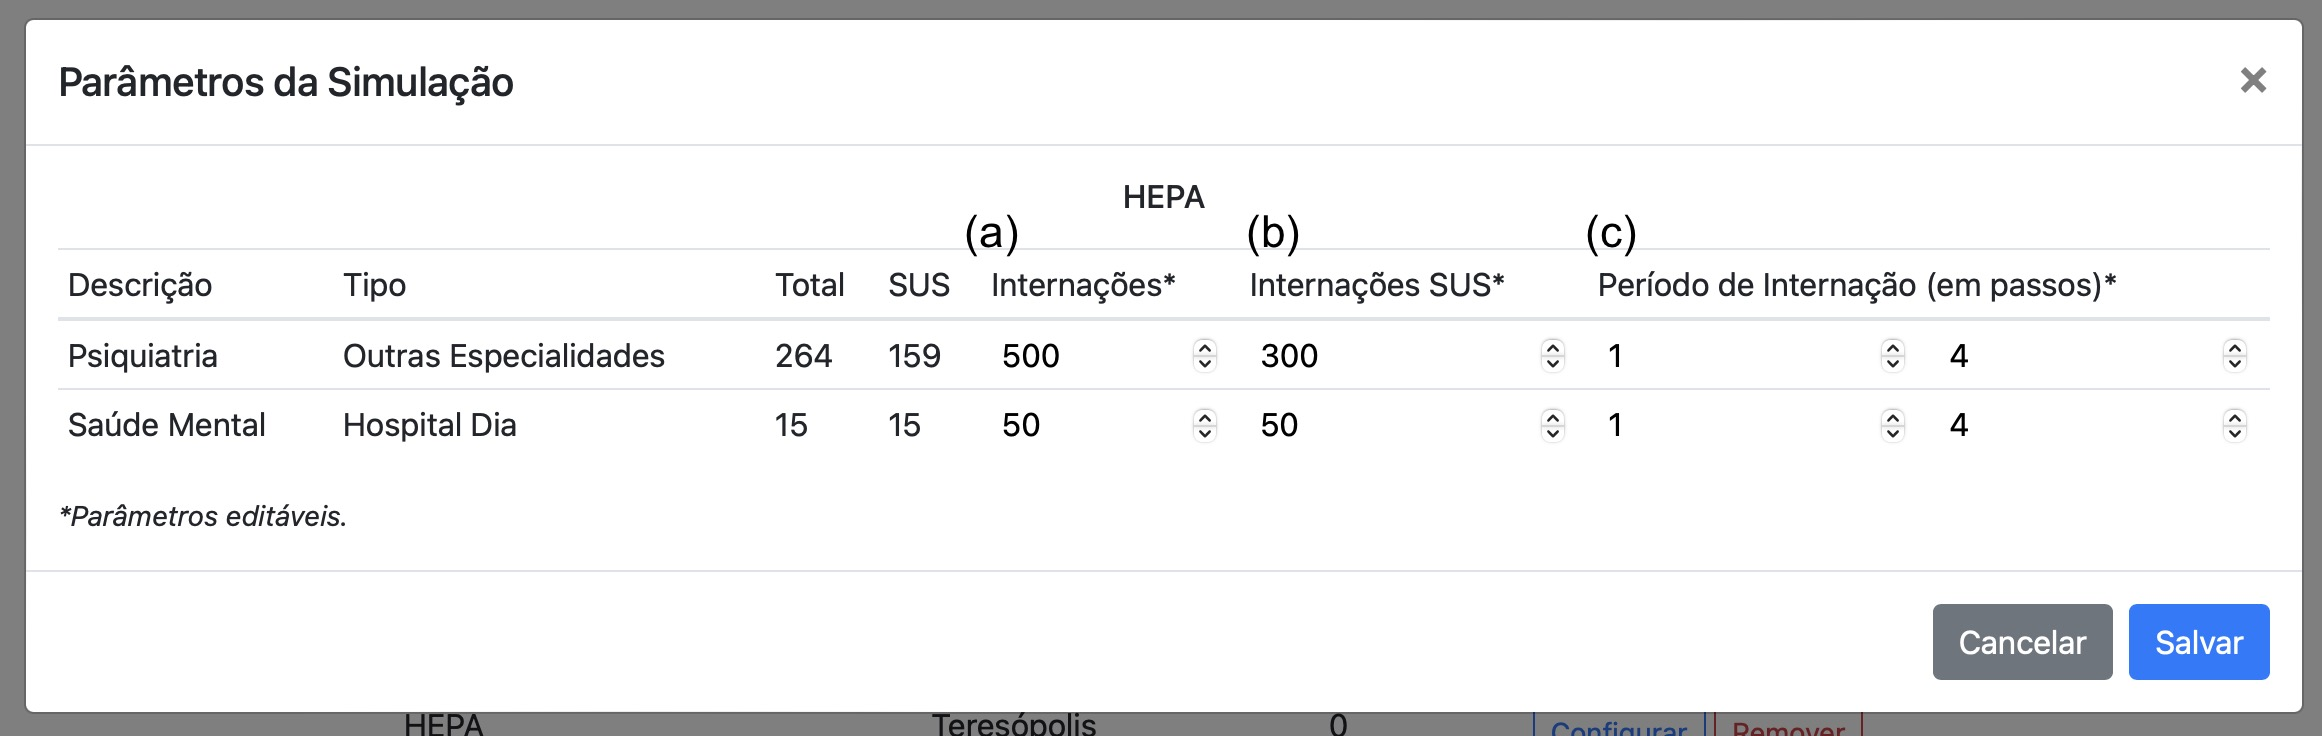
\includegraphics[width=\textwidth]{Capitulos/images/simul5.jpeg}
    \caption{Tela de parametrização da simulação.}
    \label{fig:simul5}
\end{figure}

Finalmente, ao clicar no botão "Iniciar simulação", é gerado um arquivo JSON a ser utilizado como entrada do modelo de simulação a partir dos parâmetros configurados na interface gráfica. Inicia-se a execução do modelo de simulação e, após o término da execução, os resultados são apresentados. A Seção~\ref{sec:visualizacao_resultados} deste capitulo detalha a interface utilizada para apresentar os resultados do modelo. A Listagem~\ref{json-model} ilustra um exemplo da estrutura do arquivo JSON gerado pela etapa de parametrização do modelo. 
%SO: no listing tem que ser colocadas letrinhas (a)(b) e explicada todo o texto (GV: revisao)

\begin{listing}
\begin{minted}[frame=single,
               framesep=3mm,
               linenos=true,
               xleftmargin=21pt,
               tabsize=4]{js}
{
    "title": "Nova simulação",
    "days": 3,
    "day_duration": 4,
    "hospital_data": [
        {
            "name": "HEPA",
            "region": "Teresópolis",
            "latitude": -30.0871043,
            "longitude": -51.2089115,
            "specialties": [
                {
                    "name": "Psiquiatria",
                    "sectors": [
                        {
                            "type": "Outras Especialidades",
                            "total": "264",
                            "sus": "159"
                        }
                    ]
                },
                ...
            ]
        }
        ...
    ],
    "hospital_calls": [
        {
            "name": "HEPA",
            "total-calls": [
                {
                    "name": "Psiquiatria",
                    "type": "Outras Especialidades",
                    "admissions": "20",
                    "admissions-sus": "20",
                    "range-start": "1",
                    "range-end": "3"
                },
                ...
            ]
        }
        ...
    ]
}
\end{minted}
\caption{Exemplo arquivo JSON de entrada do modelo de simulação gerado pela interface.} 
\label{json-model}
\end{listing}
\pagebreak

O arquivo representado pela Listagem~\ref{json-model} é composto das informações a seguir. O campo ``\textit{title}'' está associado ao titulo da simulação, ``\textit{days}'' é a duração da simulação em dias, ``\textit{day\_duration}'' a duração de um dia na simulação em horas, ``\textit{hospital\_data}'' contém as informações parametrizadas relacionadas a capacidade dos leitos hospitalares de cada hospital selecionado e ``\textit{hospital\_calls}'' contém as informações relacionadas ao fluxo de pacientes nos leitos hospitalares da simulação.

\section{Plugin do LODUS}\label{sec:plugin_lodus}
A partir dos dados informados e descritos nas seções anteriores, a presente etapa apresenta o desenvolvimento de um 
\textit{plugin} para o \textit{framework} LODUS~\cite{9239083}. 
%SO: ref ao lodus (GV: corrigido)
O objetivo desse \textit{plugin} é adicionar à aplicação a capacidade de contextualizar o ambiente de simulação urbana virtual para casos de ocupação de leitos hospitalares, parte fundamental no desenvolvimento da ferramenta LODUS-Health.
%SO: acima - plugin em itálico (GV: corrigido)

Para iniciar a execução da simulação, o LODUS necessita de um arquivo de configuração com a estrutura previamente definida pelos autores do \textit{framework}, o qual pode ser alterado em ferramentas de edição de texto. Entretanto, o propósito deste trabalho também é evitar a necessidade de realizar alterações nos arquivos utilizando ferramentas de edição de texto antes da execução da simulação. Para isso, a configuração do ambiente é realizada combinando os dados dos dois arquivos necessários para a contextualização e execução. Nesse processo, utiliza-se a linguagem Python. A Listagem~\ref{input-file} abaixo demonstra um exemplo da estrutura do arquivo requisitado pela aplicação, onde, ``\textit{population\_template}'' está atribuído a uma definição de características comuns entre toda a população no modelo de simulação, ``\textit{repeating\_global\_actions}'' as ações que ocorrem na simulação em determinados períodos, ``\textit{regions}'' as configurações dos bairros da cidade dentro da simulação contendo informações como, posição geográfica, as regiões vizinhas mais próximas e os pontos de interesse dentro da região contendo informações geográficas e o tamanho da população naquele ponto.

%SO: tens que colocar (a)(b) no arquivo abaixo e explicar o listing. (GV: revisao)

\begin{listing}
\begin{minted}[frame=single,
               framesep=3mm,
               linenos=true,
               xleftmargin=21pt,
               tabsize=4]{js}
{
  "population_template": {
    "traceable_properties": {},
    "sampled_properties": {}
  },
  "repeating_global_actions": [],
  "regions": [
    {
      "name": "Independência",
      "long_lat_position": [-51.2114165227445, -30.0283138642156]
      "neighbors": [
        "Floresta",
        "Moinhos de Vento",
        ...
      ],
      "nodes": {
        "home": {
          "characteristics": {
            "long_lat_position": [-51.209426628695, -30.028013704038]
          },
          "population_groups": [
            {
              "size": 8112,
              "traceable_properties": {},
              "description": {}
            }
          ],
          "time_actions": {}
        }
      }
    }...
  ]
}

\end{minted}
\caption{Exemplo de arquivo de configuração para execução do \textit{framework} LODUS.} 
\label{input-file}
\end{listing}

Os dados de configuração dos parâmetros definidos pelo usuário na interface de configuração, apresentados na seção anterior, são incorporados à configuração do ambiente de simulação, juntamente com os dados deste arquivo necessário para a execução do ambiente de simulação. O primeiro passo dessa tarefa é a configuração dos passos de simulação, que consiste na multiplicação entre a quantidade de dias a serem simulados e a duração do dia parametrizados pelo usuário. Uma configuração de 4 dias e com 3 de duração resulta em 12 passos de simulação, por exemplo.

Seguindo na configuração do \textit{plugin}, o próximo passo é a configuração dos pontos de interesse dentro da simulação, sendo um ponto de interesse uma área dentro do ambiente de simulação na qual os grupos podem se deslocar. Para cada região, optamos por trabalhar com dois possíveis pontos de interesse na simulação, sendo eles casas e hospitais. Para ilustrar, grupos de um ou mais pacientes saem de suas casas para serem internados nos hospitais, e pacientes deixam hospitais para retornarem para suas casas após um determinado período de internação. Neste estudo, não estamos considerando que pacientes venham de outros possíveis pontos de interesse ou que venham a óbito no hospital; somente o controle do fluxo de internações é considerado, pacientes que venham a óbito ou recebam alta hospitalar são tratados apenas como uma desocupação do leito hospitalar. Para que um hospital seja reconhecido como um ponto de interesse, cada hospital selecionado no arquivo de configuração é manipulado de tal forma a ser considerado um ``nodo'' dentro de uma região, sendo ``nodos'', pontos de interesse dentro de uma região com suas características próprias. Ao final dessa junção entre os dados das duas fontes, internamente na aplicação, um ``nodo'' que caracteriza um hospital dentro de uma região possui a seguinte estrutura representada na Listagem~\ref{nodo-structure}:

\begin{listing}
\begin{minted}[frame=single,
               framesep=3mm,
               linenos=true,
               xleftmargin=21pt,
               tabsize=4]{js}     
{
    "name": "HEPA",
    "id": "5",
    "routine": {
        "name": "None",
        "actions": {}
    },
    "characteristics": {
        "long_lat_position": [
            -51.2089115,
            -30.0871043
        ],
        "hospital_bed": {
            "config": [
                {
                    "name": "Psiquiatria",
                    "sectors": [
                        {
                            "type": "Outras Especialidades",
                            "total": "264",
                            "sus": "159"
                        }
                    ]
                }...
            ],
            "calls": [
                {
                    "name": "Psiquiatria",
                    "type": "Outras Especialidades",
                    "admissions": "20",
                    "admissions-sus": "20",
                    "range-start": "1",
                    "range-end": "4",
                    "distribution": [0, 0, ..., 0],
                    "distribution-sus": [6, 2, 0, ..., 1]
                },
            ]
        }
    },
    "blobs": []
}
\end{minted}
\caption{Exemplo da estrutura interna de um nodo dentro do modelo de simulação.} 
\label{nodo-structure}
\end{listing}

A Listagem~\ref{nodo-structure} apresenta as informações que caracterizam um hospital dentro do ambiente de simulação. O campo ``\textit{name}'' refere-se ao nome do hospital, ``\textit{id}'' é um identificador único para o nodo, ``\textit{routine}'' mostra as rotinas associadas ao hospital, e ``\textit{characteristics}'' são as características que compõem o nodo, incluindo ``\textit{long\_lat\_position}'' para a posição geográfica do hospital no mapa, ``\textit{hospital\_bed}'' para as configurações de leitos do hospital, onde ``\textit{config}'' são as configurações de disponibilidade de leitos e ``\textit{calls}'' refere-se às configurações de ocupação dos leitos. O campo ``\textit{config}'' está associado a uma lista de especialidades do hospital. No exemplo, o hospital HEPA possui a especialidade ``Psiquiatria'' e o tipo de leito (\textit{sectors}) ``Outras Especialidades'', totalizando 264 leitos, sendo 159 do SUS. Em ``\textit{calls}'', há uma lista de status de ocupação dos leitos. Para a especialidade ``Psiquiatria'' do tipo ``Outras Especialidades'', serão 20 pacientes internados no período de simulação (\textit{admissions}), sendo 20 internados nos leitos SUS (\textit{admissions-sus}). Cada paciente ficará no hospital por um período de 1 a 4 passos de simulação (\textit{range-start} e \textit{range-end}). Os campos ``\textit{distribution}'' e ``\textit{distribution-sus}'' são listas do tamanho do número total de passos de simulação, onde cada índice da lista representa uma entrada de pacientes para aquele leito no passo de execução atual. Por exemplo, no passo de simulação 0, 6 pacientes chegam no leito SUS e no passo 1, chegam 2. Por fim, ``\textit{blobs}'' é a lista de grupos naquele nodo, ou seja, os grupos de pacientes que estão naquele hospital com suas características próprias.

A última etapa antes da execução da simulação é a configuração das ``\textit{repeating actions}''. Uma \textit{repeating action} é uma ação que o modelo de simulação executa em um período único ou em intervalos determinados. Para cada passo de execução, são definidos três tipos de ações no \textit{plugin}: ``\textit{patient\_call}'', ``\textit{patient\_distribution}'' e ``\textit{patient\_discharge}''. Na ação ``\textit{patient\_call}'', é feita a chamada de pacientes para dentro do hospital, ou seja, um grupo de pacientes sai de suas casas para ocuparem leitos hospitalares, a única condições de busca de pacientes é que sejam apenas os que ainda não tenham sido encaminhados a algum dos hospitais na simulação. A ação ``\textit{patient\_distribution}'' transforma o grupo de pacientes que chegaram ao hospital em pacientes individuais e atribui-se cada paciente a um leito hospitalar. Já a ação ``\textit{patient\_discharge}'' é responsável por desocupar os leitos hospitalares; ao executar a ação, o hospital remove os pacientes dos leitos e os retorna cada um para sua casa em sua região de origem, utilizando uma ação previamente disponível no \textit{framework} ``\textit{move\_population}''. Essas ações são associadas a cada hospital que estiver parametrizado na simulação. Em cada passo de execução, os hospitais recebem e retornam pacientes.

Após a estruturação do modelo, a etapa seguinte é a execução da simulação. Para cada passo de simulação, a ação ``\textit{patient\_call}'' aumenta a quantidade de pacientes internados no hospital. Para cada especialidade, verificam-se os campos ``\textit{distribution}'' e ``\textit{distribution-sus}'' para contabilizar o número de pacientes a serem internados naquele passo de execução, soma se cada quantidade e é feito a chamada de um grupo de pacientes para o hospital considerando o valor total da soma. Para a chamada de pacientes, considera-se apenas aqueles que ainda não foram internados até o passo de simulação atual.

Na ação ``\textit{patient\_distribution}'', o grupo de pacientes retornados na ação anterior é associado a pacientes únicos. Cada paciente recebe um identificador único (\textit{patient\_id}), a região de onde o paciente veio (\textit{from\_region}), a especialidade do leito de internação (\textit{specialty}), o tipo de leito (\textit{type}), e um tempo de permanência aleatório (\textit{admission\_time}) dentro do intervalo de entrada e saída definido pelo usuário na configuração. O passo de simulação em que o paciente vai deixar o hospital (\textit{return\_frame}) é determinado pela soma do passo atual mais o tempo de permanência. Por fim, é informado se o paciente está em um leito SUS ou não (\textit{is\_sus}). A Listagem~\ref{lst:pacient_estru} mostra um exemplo da estrutura de um paciente dentro do modelo de simulação.

\begin{listing}
\begin{minted}[frame=single,
               framesep=3mm,
               linenos=true,
               xleftmargin=21pt,
               tabsize=4]{js}     
{
   'patient_id': 'e03b4d75-c3d2-4ed7-976e-f44925e27796', 
   'from_region': 'Teresópolis', 
   'specialty': 'Saúde Mental', 
   'type': 'Hospital Dia', 
   'admission_time': 1, 
   'return_frame': 1, 
   'is_sus': True
}
\end{minted}
\caption{Exemplo da estrutura de um paciente na simulação.} 
\label{lst:pacient_estru}
\end{listing}

Por fim, a ação ``\textit{patient\_discharge}'' é responsável por liberar os pacientes dos leitos hospitalares. Para isso, é feito uma verificação em cada um dos pacientes internados se o passo de simulação atual é igual a seu ``\textit{return\_frame}'', caso seja, o paciente é retornado para sua casa na sua região de origem associada no campo ``\textit{from\_region}''. A execução dessa ação ocorre durante todos os passos de execução, e em cada passo, são armazenadas as informações do estado atual dos leitos hospitalares na simulação. A Tabela~\ref{table:passos} mostra um exemplo desse arquivo que será utilizado para apresentar os resultados da simulação posteriormente na interface gráfica, no arquivo está representado os estados dos leitos do hospital HEPA por três passos de simulação. Cada entrada do arquivo é compostas das informações de ``\textit{Frame}'', que está associado ao passo de simulação, ``\textit{Hour}'' ao horário dentro do dia, ``\textit{Day}'' ao dia de simulação, ``\textit{Hospital}'' ao nome do hospital, ``\textit{Bed}'' à especialidade, ``\textit{Type}'' ao tipo de leito, ``\textit{total}'' ao total de pacientes naquele leito, ``\textit{Total\_SUS}'' ao total de pacientes nos leitos SUS entre o total de leitos e ``\textit{Patient\_data}'' a uma lista dos pacientes internados naquela especialidade no passo de simulação atual. O Algoritmo~\ref{alg:algo} demonstra como é feita a lógica de internação dos pacientes nos leitos hospitalares dentro do modelo de simulação.

\begin{table}[!ht]
    \centering
    \begin{tabular}{p{0.05\textwidth}p{0.03\textwidth}p{0.02\textwidth}p{0.11\textwidth}p{0.07\textwidth}p{0.1\textwidth}p{0.1\textwidth}p{0.03\textwidth}p{0.1\textwidth}p{0.1\textwidth}}
        Frame & Hour & Day & Region & Hospital & Bed & Type & Total & Total\_SUS & Patient\_Data \\ \hline
        0 & 0 & 0 & Teresópolis & HEPA & Psiquiatria & Outras Especi... & 6 & 6 & [\{'patient\_id': 'e03b...]\\
        0 & 0 & 0 & Teresópolis & HEPA & Saúde Mental & Hospital Dia & 5 & 4 & [\{'patient\_id': '3851...]\\
        1 & 1 & 0 & Teresópolis & HEPA & Psiquiatria & Outras Especi... & 7 & 7 & [\{'patient\_id': 'ce52...]\\
        1 & 1 & 0 & Teresópolis & HEPA & Saúde Mental & Hospital Dia & 3 & 3 & [\{'patient\_id': '3851...]\\
        2 & 2 & 0 & Teresópolis & HEPA & Psiquiatria & Outras Especi... & 1 & 1 & [\{'patient\_id': 'ce521...]\\
        2 & 2 & 0 & Teresópolis & HEPA & Saúde Mental & Hospital Dia & 5 & 4 & [\{'patient\_id': '3851...]\\
    \end{tabular}
    \caption{Registros dos passos de execução da simulação.}
    \label{table:passos}
\end{table}

\begin{algorithm}[H] 
\begin{algorithmic}[1]
\Require{$N$ (quantidade de pacientes)} 
\Require{$inicio$ (tempo mínimo de permanecia)} 
\Require{$fim$ (tempo máximo de permanecia)} 
\Require{$passo$ (passo atual)} 
% \Require{$L_{1} \dots L_{M}$ (lista de passos de simulação)} 
\Statex
\Function{distribuiPacientes}{$ $}
    \For{$k \gets 1$ ate $N$}                    
        \State {$tempoPermanencia \gets sorteiaTempoPermanencia(inicio,fim)$}
        \State {$passoRetorno$ $\gets$ {$passo + tempoPermanencia$}}
        \State {$paciente$ $\gets$ $criaPaciente(tempoPermanencia, passoRetorno)$}
        \State {$atribuiPacienteAoHospital(paciente)$}
    \EndFor
\EndFunction
\end{algorithmic}
\caption{Distribuição de pacientes no hospital.}
\label{alg:algo}
\end{algorithm}

\section{Visualização dos Resultados}\label{sec:visualizacao_resultados}
Inicialmente, para o desenvolvimento da interface de visualização dos resultados, foi necessário a criação da geometria dos bairros da cidade de Porto Alegre para visualização dos dados geoespaciais em um mapa na aplicação. Para isso, utilizou-se da demarcação de território dos bairros da cidade disponibilizada no site da prefeitura\footnote{\url{https://prefeitura.poa.br/carta-de-servicos/mapas-digitais-da-smamus}}, essa demarcação é disponibilizada como um arquivo \textit{shapefile} e convertido para o formato geoJSON com a ferramenta QGIS\footnote{\url{https://qgis.org/pt_BR/site/forusers/download.html}}. A ferramenta web GeoJson.io\footnote{\url{https://geojson.io/}} é utilizada para validação das coordenadas geográficas geradas pelo QGIS. Figura~\ref{fig:geojson} mostra a interface da ferramenta GeoJson.io na apresentação da geometria dos bairros de Porto Alegre.
%GA: colocar a fonte dos dados para a geometria dos bairros: https://prefeitura.poa.br/carta-de-servicos/mapas-digitais-da-smamus. É um arquivo shapefile q foi convertido para geoJSON com o Q-GIS (GV: corrigido)

\begin{figure}
    \centering
    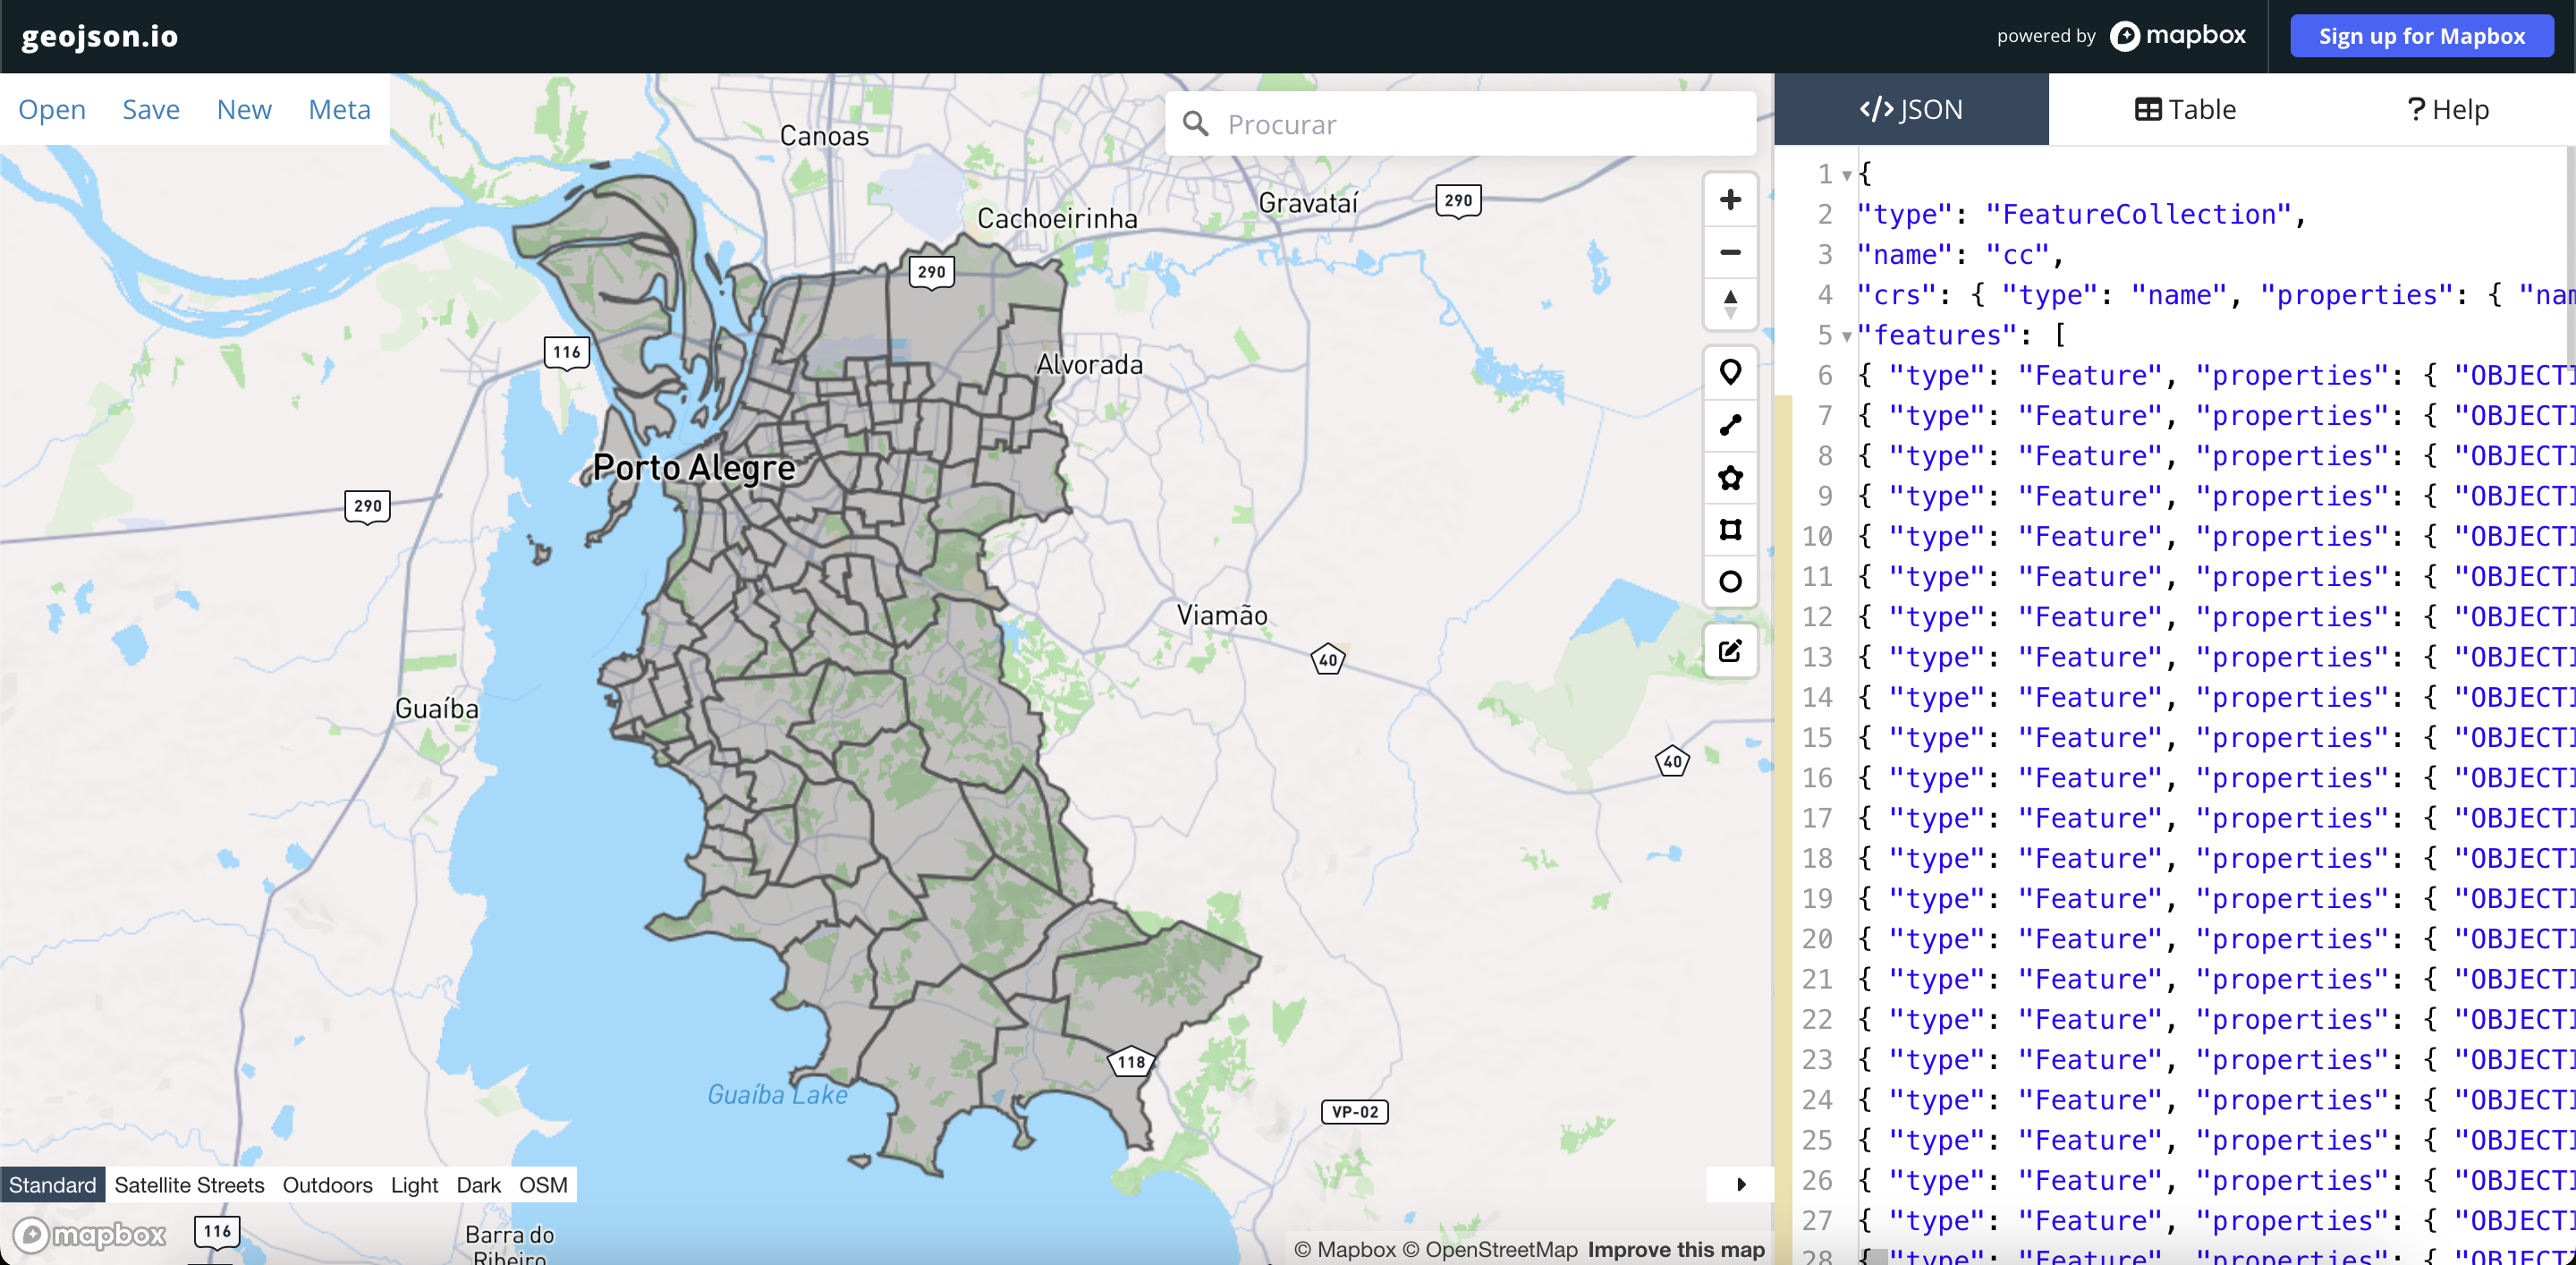
\includegraphics[width=\textwidth]{Capitulos/images/geojson.png}
    \caption{Visualização das coordenadas da cidade de Porto Alegre na aplicação GeoJson.io com os dados gerados na ferramenta QGIS.
    %GA: essa tela é só a visualização dos dados da prefeitura que tem os contorno dos bairros, certo? se não tem resultados da simulação nem criação desses dados, ajustar a legenda (GV: corrigido)
    }
    \label{fig:geojson}
\end{figure}

A apresentação dos resultados obtidos na simulação faz parte da mesma aplicação de interface gráfica utilizada na geração dos parâmetros do modelo de simulação. A tela inicial da apresentação dos resultados (Figura~\ref{fig:result_simulacao_1}) permite que o usuário interaja com duas ações: escolhendo o dia e hora (passo) da simulação para visualizar os resultados (Figura~\ref{fig:result_simulacao_1}(a)) e selecionando um bairro no mapa para obter informações detalhadas sobre os hospitais daquele bairro no passo de simulação selecionado (Figura~\ref{fig:result_simulacao_1}(b)). As cores no mapa representam a lotação geral dos hospitais naquele bairro, onde as cores de tom verde representam pouco uso dos leitos e as de tom vermelho representa superlotação dos leitos. No contexto da Figura~\ref{fig:result_simulacao_1} estão presentes hospitais em duas regiões simuladas, Teresópolis e Agronomia, no tempo de simulação do dia 0 e hora 0 eles apresentam um baixo uso dos leitos (tons verdes).

\begin{figure}
    \centering
    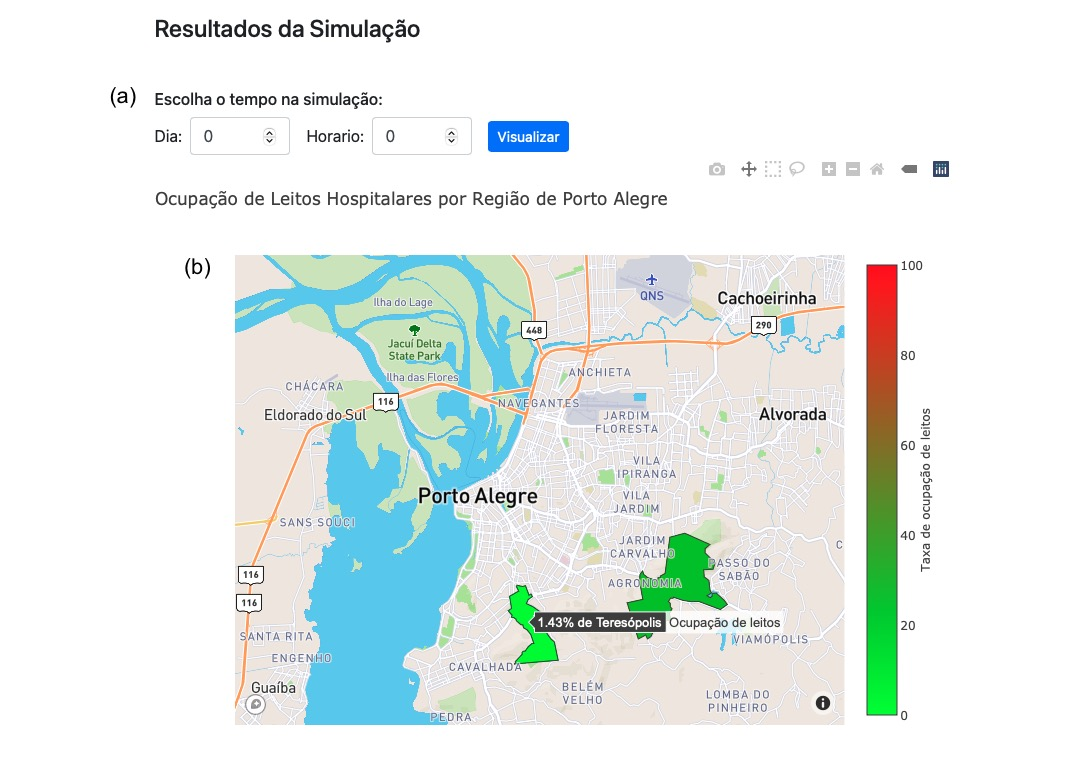
\includegraphics[width=\textwidth]{Capitulos/images/result1.jpeg}
    \caption{Tela inicial dos resultados da simulação.}
    \label{fig:result_simulacao_1}
\end{figure}

Ao selecionar um bairro no mapa, estão disponíveis informações relacionadas à lotação dos leitos hospitalares. A Figura~\ref{fig:result2} apresenta essas informações. Para cada hospital da região, estão disponíveis as seguintes informações: nome do hospital (Figura~\ref{fig:result2}(a)), porcentagem da ocupação total de leitos e dos leitos SUS (Figura~\ref{fig:result2}(b)), lista de ocupação das especialidades do hospital (Figura~\ref{fig:result2}(c)) e a opção de geração de texto para aquela especialidade (Figura~\ref{fig:result2}(d)). No exemplo, estão sendo apresentadas as informações do hospital HEPA do bairro Teresópolis, o hospital tem 1,43\% da ocupação total dos leitos utilizada e 2,3\% dos leitos SUS, abaixo apresenta os dados de cada especialidade de leito individualmente, para o leito ``Psquiatria'' do tipo ``Outras especialidades'' estão sendo utilizados 3 leitos, sendo os 3 leitos SUS e para a especialidade ``Saúde Mental'' do tipo ``Hospital Dia'' está sendo utilizado 1 leito e também sendo um leito SUS. A seção a seguir vai apresentar o processo de geração de texto médico (Figura~\ref{fig:result2}(d)) como exemplo para uma determinada especialidade.

%GA: acho que aqui cabe uma colinha melhor com a proxima section, ja que ela é um pouco diferente do resto (GV: corrigido)

\begin{figure}
    \centering
    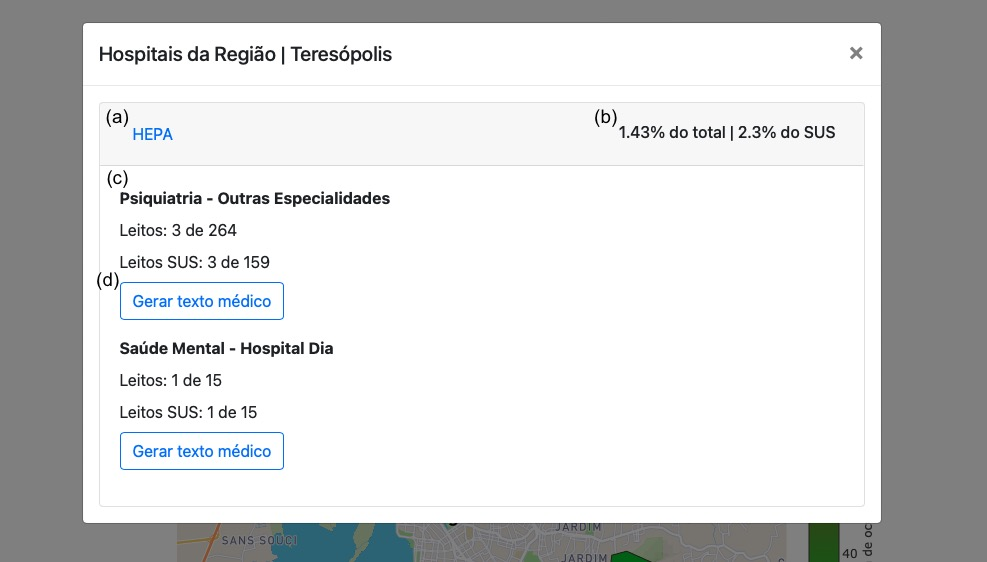
\includegraphics[width=\textwidth]{Capitulos/images/result2.jpeg}
    \caption{Resultados de um passo simulação em um bairro selecionado.}
    \label{fig:result2}
\end{figure}


\section{Geração de Texto Médico Individualizado}\label{sec:geracao_texto}
Para a geração de texto médico (Figura~\ref{fig:result2}(d)), utilizou-se da OpenAI API, apresentada na Seção~\ref{sec:chat}. Ao clicar no botão ``Gerar texto médico'', dispara-se um evento de comunicação com a API utilizando a seguinte estrutura de \textit{prompt}, definida com o auxílio de profissionais da área da medicina:

%GA: colocar o texto abaixo em um verbatim ou alguma extrutura diferenciada, esta mt similar ao texto mas não pertence diretamente a ele
\begin{spverbatim}
Imagine que você é um médico trabalhando no hospital na emergência. Você é 
responsável por atender os pacientes que chegam via emergência para 
especialidade ``(ESPECIALIDADE)'' do tipo ``(TIPO DE ESPECIALIDADE)'' para 
internação em um leito (SUS), que apresentam  diferentes apresentações 
e diagnósticos, desde quadros leves quanto quadros graves. Você faz a primeira 
avaliação médica, que abrange a anamnese e o exame físico. Após avaliar 
o paciente você decide as condutas que devem ser tomadas para internação do 
paciente, quais os próximos passos a serem feitos. Você precisa registrar essa 
avaliação médica no prontuário do paciente, ou seja, você precisa evoluir o 
paciente no sistema. Essa evolução deve ser sucinta, usando siglas médicas 
quando adequado e deve incluir os seguintes tópicos:

Nome do setor que você está atendendo em MAIÚSCULO.
O identificador do paciente deve ser: (IDENTIFICADOR)
Lista de problemas do paciente. Aqui você deve citar:
Os problemas de saúde prévios do paciente.
Medicações em uso de o paciente fizer uso de algum medicamento de uso contínuo
Uso de drogas: escrever se paciente fuma, bebe usa outras drogas ou não. Pode 
descrever a carga tabágica em maços/ano do paciente se ele for fumante.
HDA: História da doença atual
Aqui você deve escrever de forma sucinta o motivo que fez o paciente procurar 
atendimento médico.
Subjetivo: Aqui você deve escrever as informações relatadas pelo paciente ou 
familiar que sejam relevantes sobre a história do adoecimento. Como por 
exemplo, quando o quadro começou, quais os sintomas e sinais associados, como 
evoluiu até a procura do atendimento médico e etc.
Objetivo: Aqui você deve escrever o exame físico do paciente de forma sucinta 
e composto no mínimo por: Estado geral do paciente, avaliação do sensório, ausculta cardíaca, ausculta pulmonar, abdômen, extremidades.
Pode conter também outras informações conforme sejam necessárias a avaliação 
clinica conforme o quadro do paciente, como avaliação de deficit de força no 
avc, pele em afecções dermatológicas, etc. Você como médico deve buscar no 
exame físico do paciente achados que sejam relevantes para o quadro do 
paciente.
Logo abaixo do objetivo ou antes, você pode descrever resultados de exames 
laboratoriais e/ou de imagem do paciente que tenham sido realizados para 
avaliação do quadro dele. Anote sempre o nome do exame e a data da realização 
dele.
Impressão: Aqui você deve escrever as suas impressões gerais do quadro do 
paciente, como diagnósticos possíveis, gravidade
Conduta: aqui você deve listar as suas ações tomadas como médico, ou seja, as 
condutas que você tomou. Por exemplo: medicamentos prescritos ou removidos, 
solicitação de exames, consultoria com especialistas, descrição sucinta de 
conversas com familiares ou outros membros da equipe assistencial, Orientações 
para a alta se houverem, encaminhamentos, transferências.
\end{spverbatim}
%SO: achei que o texto acima poderia estar dentro de um quadro, outra fonte... sei lá... (GV: corrigido)

%SO: abaico tem figura para ilustrar essa parte?
Pela utilização da interface gráfica, o usuário pode definir o contexto do texto a ser gerado, ou seja, dentre as opções de leitos configuradas, o usuário seleciona qual especialidade e tipo de leito deseja retornar gerar exemplos de texto de evolução de pacientes (Figura~\ref{fig:result2}). Ao selecionar, é sorteado algum dos pacientes que estão internados no hospital naquela especialidade de leito e os campos (ESPECIALIDADE), (TIPO DE ESPECIALIDADE), (SUS) e (IDENTIFICADOR) do texto acima são substituídos pelas informações do paciente no contexto selecionado, a seguir é enviado como \textit{prompt} para a API. Abaixo se tem um exemplo de uma geração de texto para a especialidade ``Psiquiatria'' do tipo de leito ``Outras Especialidades'' atribuído a um leito privado.

\begin{spverbatim}
SETOR DE EMERGÊNCIA PSIQUIÁTRICA

IDENTIFICADOR DO PACIENTE: b4555eab-2565-4a22-ac22-028fe7bb9f38

Lista de Problemas:
- Saúde Prévia: Diabetes tipo 2 em tratamento com metformina.
- Medicações em Uso: Metformina 850mg, 1 comprimido duas vezes ao dia.
- Uso de Drogas: Nega tabagismo, consumo moderado de álcool socialmente.

HDA (História da Doença Atual):
Paciente apresenta quadro de agitação psicomotora e alucinações auditivas há 2 dias.

Subjetivo:
Relatado pela paciente: Início gradual dos sintomas, piora progressiva da agitação e desconforto psíquico associado às vozes que ouve.

Objetivo:
- Estado Geral: Paciente agitada, inquieta, olhar ansioso.
- Avaliação do Sensório: Desorientada no tempo, alerta quanto a pessoa e lugar.
- Ausculta Cardíaca: Ritmo cardíaco regular, sem sopros.
- Ausculta Pulmonar: Murmúrios vesiculares presentes bilateralmente.
- Abdômen: Macio, indolor à palpação, sem visceromegalias.
- Extremidades: Sem edemas ou sinais de trombose venosa profunda.

Resultados de Exames:
- Eletrocardiograma (ECG) realizado em 05/04/2024: Sem alterações significativas.

Impressão:
Possível episódio de psicose aguda em contexto de diabetes descompensada.

Conduta:
1. Prescrição de haloperidol 5mg via intramuscular para controle da agitação.
2. Solicitação de glicemia capilar para avaliação da glicemia atual.
3. Comunicação com a equipe de endocrinologia para avaliação e ajuste do tratamento antidiabético.
4. Orientação para acompanhamento psiquiátrico após a estabilização do quadro agudo.
5. Discussão do caso com equipe multidisciplinar para monitoramento contínuo da paciente.

Registro realizado em 05/04/2024.
\end{spverbatim}

Nos próximos capítulos serão analisados e discutidos os resultados de diferentes contextos de simulação utilizando o modelo apresentado nesse capitulo.

%SO: Faltou explicar como selecionaste o indivídulo. Da fig 4.15, tem vários leit0s.... de quem geraste? todos? como selecionas? (GV: revisao)

%SO: ainda aqui, é legal mostrar um exemplod e geração, não terminar tão bruscamente o capítulo. E indicar, ao final do capítulo, que no próximo serão analisados e discutidos os resutlados... (GV: corrigido)

%GA: se tu conseguir montar um video curto (captura de tela mesmo) do processo de montagem da simulação, executar e ver os resultados, isso pode virar um footnote no final desse capitulo